% Created by tikzDevice version 0.12.3.1 on 2023-02-23 13:43:11
% !TEX encoding = UTF-8 Unicode
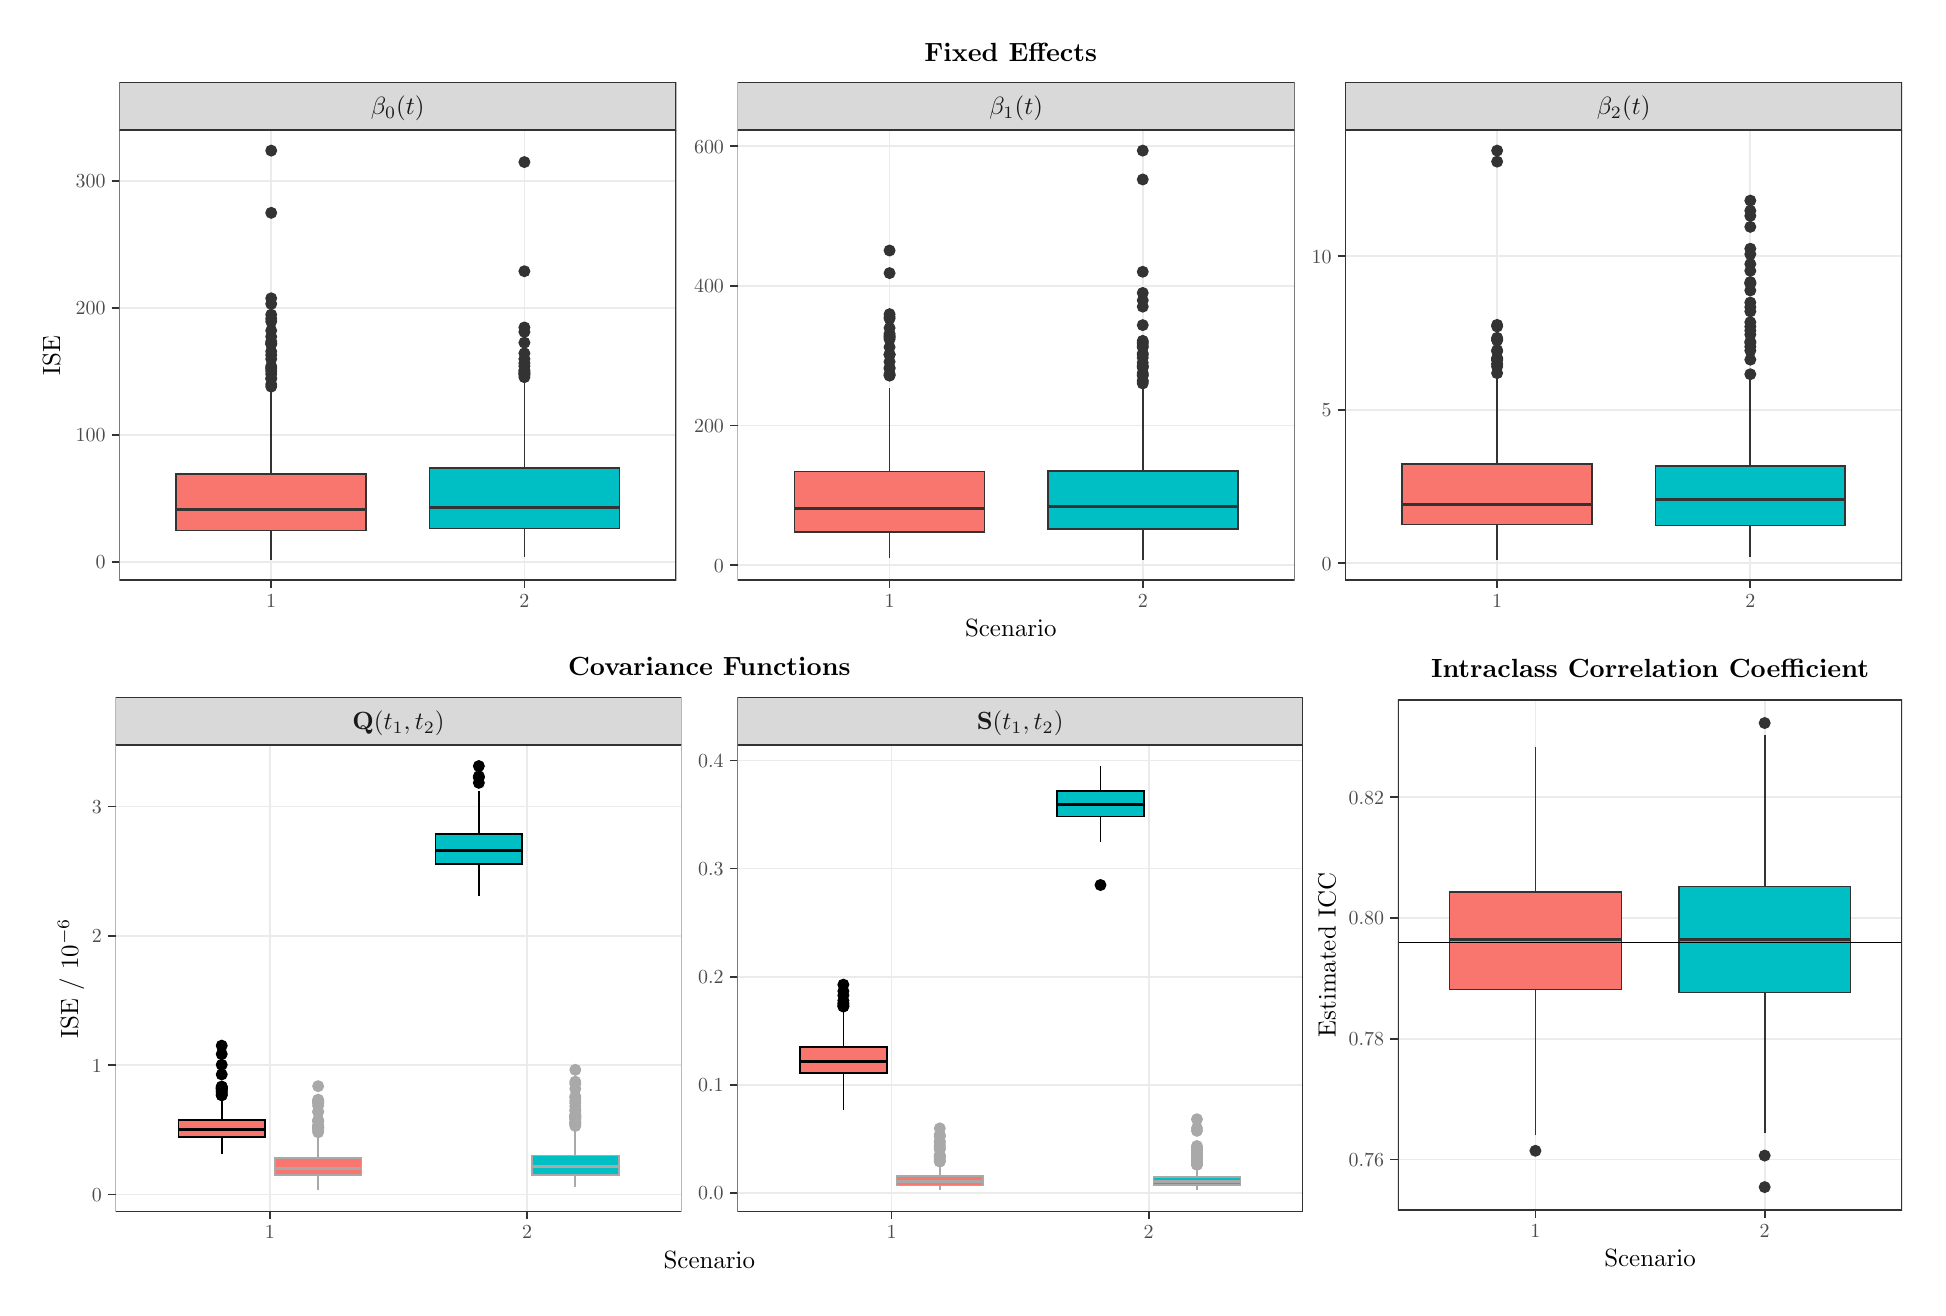
\begin{tikzpicture}[x=1pt,y=1pt]
\definecolor{fillColor}{RGB}{255,255,255}
\path[use as bounding box,fill=fillColor,fill opacity=0.00] (0,0) rectangle (682.86,455.24);
\begin{scope}
\path[clip] (  0.00,227.62) rectangle (682.86,455.24);
\definecolor{drawColor}{RGB}{255,255,255}
\definecolor{fillColor}{RGB}{255,255,255}

\path[draw=drawColor,line width= 0.6pt,line join=round,line cap=round,fill=fillColor] (  0.00,227.62) rectangle (682.86,455.24);
\end{scope}
\begin{scope}
\path[clip] ( 33.11,255.60) rectangle (234.38,418.21);
\definecolor{fillColor}{RGB}{255,255,255}

\path[fill=fillColor] ( 33.11,255.60) rectangle (234.38,418.21);
\definecolor{drawColor}{gray}{0.92}

\path[draw=drawColor,line width= 0.6pt,line join=round] ( 33.11,262.26) --
	(234.38,262.26);

\path[draw=drawColor,line width= 0.6pt,line join=round] ( 33.11,308.12) --
	(234.38,308.12);

\path[draw=drawColor,line width= 0.6pt,line join=round] ( 33.11,353.98) --
	(234.38,353.98);

\path[draw=drawColor,line width= 0.6pt,line join=round] ( 33.11,399.85) --
	(234.38,399.85);

\path[draw=drawColor,line width= 0.6pt,line join=round] ( 88.00,255.60) --
	( 88.00,418.21);

\path[draw=drawColor,line width= 0.6pt,line join=round] (179.49,255.60) --
	(179.49,418.21);
\definecolor{drawColor}{gray}{0.20}
\definecolor{fillColor}{gray}{0.20}

\path[draw=drawColor,line width= 0.4pt,line join=round,line cap=round,fill=fillColor] ( 88.00,341.16) circle (  1.96);

\path[draw=drawColor,line width= 0.4pt,line join=round,line cap=round,fill=fillColor] ( 88.00,351.52) circle (  1.96);

\path[draw=drawColor,line width= 0.4pt,line join=round,line cap=round,fill=fillColor] ( 88.00,328.55) circle (  1.96);

\path[draw=drawColor,line width= 0.4pt,line join=round,line cap=round,fill=fillColor] ( 88.00,357.44) circle (  1.96);

\path[draw=drawColor,line width= 0.4pt,line join=round,line cap=round,fill=fillColor] ( 88.00,332.32) circle (  1.96);

\path[draw=drawColor,line width= 0.4pt,line join=round,line cap=round,fill=fillColor] ( 88.00,349.05) circle (  1.96);

\path[draw=drawColor,line width= 0.4pt,line join=round,line cap=round,fill=fillColor] ( 88.00,345.80) circle (  1.96);

\path[draw=drawColor,line width= 0.4pt,line join=round,line cap=round,fill=fillColor] ( 88.00,340.93) circle (  1.96);

\path[draw=drawColor,line width= 0.4pt,line join=round,line cap=round,fill=fillColor] ( 88.00,338.26) circle (  1.96);

\path[draw=drawColor,line width= 0.4pt,line join=round,line cap=round,fill=fillColor] ( 88.00,336.95) circle (  1.96);

\path[draw=drawColor,line width= 0.4pt,line join=round,line cap=round,fill=fillColor] ( 88.00,328.36) circle (  1.96);

\path[draw=drawColor,line width= 0.4pt,line join=round,line cap=round,fill=fillColor] ( 88.00,325.53) circle (  1.96);

\path[draw=drawColor,line width= 0.4pt,line join=round,line cap=round,fill=fillColor] ( 88.00,350.13) circle (  1.96);

\path[draw=drawColor,line width= 0.4pt,line join=round,line cap=round,fill=fillColor] ( 88.00,410.81) circle (  1.96);

\path[draw=drawColor,line width= 0.4pt,line join=round,line cap=round,fill=fillColor] ( 88.00,330.01) circle (  1.96);

\path[draw=drawColor,line width= 0.4pt,line join=round,line cap=round,fill=fillColor] ( 88.00,335.50) circle (  1.96);

\path[draw=drawColor,line width= 0.4pt,line join=round,line cap=round,fill=fillColor] ( 88.00,331.87) circle (  1.96);

\path[draw=drawColor,line width= 0.4pt,line join=round,line cap=round,fill=fillColor] ( 88.00,343.57) circle (  1.96);

\path[draw=drawColor,line width= 0.4pt,line join=round,line cap=round,fill=fillColor] ( 88.00,331.05) circle (  1.96);

\path[draw=drawColor,line width= 0.4pt,line join=round,line cap=round,fill=fillColor] ( 88.00,388.33) circle (  1.96);

\path[draw=drawColor,line width= 0.4pt,line join=round,line cap=round,fill=fillColor] ( 88.00,332.92) circle (  1.96);

\path[draw=drawColor,line width= 0.4pt,line join=round,line cap=round,fill=fillColor] ( 88.00,340.93) circle (  1.96);

\path[draw=drawColor,line width= 0.4pt,line join=round,line cap=round,fill=fillColor] ( 88.00,326.35) circle (  1.96);

\path[draw=drawColor,line width= 0.4pt,line join=round,line cap=round,fill=fillColor] ( 88.00,341.83) circle (  1.96);

\path[draw=drawColor,line width= 0.4pt,line join=round,line cap=round,fill=fillColor] ( 88.00,355.42) circle (  1.96);

\path[draw=drawColor,line width= 0.6pt,line join=round] ( 88.00,294.03) -- ( 88.00,324.57);

\path[draw=drawColor,line width= 0.6pt,line join=round] ( 88.00,273.50) -- ( 88.00,262.99);
\definecolor{fillColor}{RGB}{248,118,109}

\path[draw=drawColor,line width= 0.6pt,fill=fillColor] ( 53.69,294.03) --
	( 53.69,273.50) --
	(122.31,273.50) --
	(122.31,294.03) --
	( 53.69,294.03) --
	cycle;

\path[draw=drawColor,line width= 1.1pt] ( 53.69,281.27) -- (122.31,281.27);
\definecolor{fillColor}{gray}{0.20}

\path[draw=drawColor,line width= 0.4pt,line join=round,line cap=round,fill=fillColor] (179.49,330.13) circle (  1.96);

\path[draw=drawColor,line width= 0.4pt,line join=round,line cap=round,fill=fillColor] (179.49,341.42) circle (  1.96);

\path[draw=drawColor,line width= 0.4pt,line join=round,line cap=round,fill=fillColor] (179.49,330.52) circle (  1.96);

\path[draw=drawColor,line width= 0.4pt,line join=round,line cap=round,fill=fillColor] (179.49,328.94) circle (  1.96);

\path[draw=drawColor,line width= 0.4pt,line join=round,line cap=round,fill=fillColor] (179.49,345.31) circle (  1.96);

\path[draw=drawColor,line width= 0.4pt,line join=round,line cap=round,fill=fillColor] (179.49,406.67) circle (  1.96);

\path[draw=drawColor,line width= 0.4pt,line join=round,line cap=round,fill=fillColor] (179.49,337.57) circle (  1.96);

\path[draw=drawColor,line width= 0.4pt,line join=round,line cap=round,fill=fillColor] (179.49,332.93) circle (  1.96);

\path[draw=drawColor,line width= 0.4pt,line join=round,line cap=round,fill=fillColor] (179.49,330.97) circle (  1.96);

\path[draw=drawColor,line width= 0.4pt,line join=round,line cap=round,fill=fillColor] (179.49,331.53) circle (  1.96);

\path[draw=drawColor,line width= 0.4pt,line join=round,line cap=round,fill=fillColor] (179.49,346.91) circle (  1.96);

\path[draw=drawColor,line width= 0.4pt,line join=round,line cap=round,fill=fillColor] (179.49,367.23) circle (  1.96);

\path[draw=drawColor,line width= 0.4pt,line join=round,line cap=round,fill=fillColor] (179.49,329.77) circle (  1.96);

\path[draw=drawColor,line width= 0.4pt,line join=round,line cap=round,fill=fillColor] (179.49,335.52) circle (  1.96);

\path[draw=drawColor,line width= 0.4pt,line join=round,line cap=round,fill=fillColor] (179.49,334.02) circle (  1.96);

\path[draw=drawColor,line width= 0.6pt,line join=round] (179.49,296.08) -- (179.49,328.23);

\path[draw=drawColor,line width= 0.6pt,line join=round] (179.49,274.27) -- (179.49,263.94);
\definecolor{fillColor}{RGB}{0,191,196}

\path[draw=drawColor,line width= 0.6pt,fill=fillColor] (145.18,296.08) --
	(145.18,274.27) --
	(213.80,274.27) --
	(213.80,296.08) --
	(145.18,296.08) --
	cycle;

\path[draw=drawColor,line width= 1.1pt] (145.18,282.00) -- (213.80,282.00);

\path[draw=drawColor,line width= 0.6pt,line join=round,line cap=round] ( 33.11,255.60) rectangle (234.38,418.21);
\end{scope}
\begin{scope}
\path[clip] (256.55,255.60) rectangle (457.83,418.21);
\definecolor{fillColor}{RGB}{255,255,255}

\path[fill=fillColor] (256.55,255.60) rectangle (457.83,418.21);
\definecolor{drawColor}{gray}{0.92}

\path[draw=drawColor,line width= 0.6pt,line join=round] (256.55,261.02) --
	(457.83,261.02);

\path[draw=drawColor,line width= 0.6pt,line join=round] (256.55,311.48) --
	(457.83,311.48);

\path[draw=drawColor,line width= 0.6pt,line join=round] (256.55,361.94) --
	(457.83,361.94);

\path[draw=drawColor,line width= 0.6pt,line join=round] (256.55,412.40) --
	(457.83,412.40);

\path[draw=drawColor,line width= 0.6pt,line join=round] (311.44,255.60) --
	(311.44,418.21);

\path[draw=drawColor,line width= 0.6pt,line join=round] (402.93,255.60) --
	(402.93,418.21);
\definecolor{drawColor}{gray}{0.20}
\definecolor{fillColor}{gray}{0.20}

\path[draw=drawColor,line width= 0.4pt,line join=round,line cap=round,fill=fillColor] (311.44,329.62) circle (  1.96);

\path[draw=drawColor,line width= 0.4pt,line join=round,line cap=round,fill=fillColor] (311.44,350.77) circle (  1.96);

\path[draw=drawColor,line width= 0.4pt,line join=round,line cap=round,fill=fillColor] (311.44,366.55) circle (  1.96);

\path[draw=drawColor,line width= 0.4pt,line join=round,line cap=round,fill=fillColor] (311.44,374.71) circle (  1.96);

\path[draw=drawColor,line width= 0.4pt,line join=round,line cap=round,fill=fillColor] (311.44,344.01) circle (  1.96);

\path[draw=drawColor,line width= 0.4pt,line join=round,line cap=round,fill=fillColor] (311.44,332.02) circle (  1.96);

\path[draw=drawColor,line width= 0.4pt,line join=round,line cap=round,fill=fillColor] (311.44,351.73) circle (  1.96);

\path[draw=drawColor,line width= 0.4pt,line join=round,line cap=round,fill=fillColor] (311.44,332.40) circle (  1.96);

\path[draw=drawColor,line width= 0.4pt,line join=round,line cap=round,fill=fillColor] (311.44,337.17) circle (  1.96);

\path[draw=drawColor,line width= 0.4pt,line join=round,line cap=round,fill=fillColor] (311.44,346.72) circle (  1.96);

\path[draw=drawColor,line width= 0.4pt,line join=round,line cap=round,fill=fillColor] (311.44,337.09) circle (  1.96);

\path[draw=drawColor,line width= 0.4pt,line join=round,line cap=round,fill=fillColor] (311.44,342.63) circle (  1.96);

\path[draw=drawColor,line width= 0.4pt,line join=round,line cap=round,fill=fillColor] (311.44,330.14) circle (  1.96);

\path[draw=drawColor,line width= 0.4pt,line join=round,line cap=round,fill=fillColor] (311.44,334.54) circle (  1.96);

\path[draw=drawColor,line width= 0.4pt,line join=round,line cap=round,fill=fillColor] (311.44,343.22) circle (  1.96);

\path[draw=drawColor,line width= 0.4pt,line join=round,line cap=round,fill=fillColor] (311.44,337.09) circle (  1.96);

\path[draw=drawColor,line width= 0.4pt,line join=round,line cap=round,fill=fillColor] (311.44,343.59) circle (  1.96);

\path[draw=drawColor,line width= 0.4pt,line join=round,line cap=round,fill=fillColor] (311.44,350.09) circle (  1.96);

\path[draw=drawColor,line width= 0.4pt,line join=round,line cap=round,fill=fillColor] (311.44,344.65) circle (  1.96);

\path[draw=drawColor,line width= 0.4pt,line join=round,line cap=round,fill=fillColor] (311.44,339.82) circle (  1.96);

\path[draw=drawColor,line width= 0.4pt,line join=round,line cap=round,fill=fillColor] (311.44,329.49) circle (  1.96);

\path[draw=drawColor,line width= 0.6pt,line join=round] (311.44,294.86) -- (311.44,325.21);

\path[draw=drawColor,line width= 0.6pt,line join=round] (311.44,272.88) -- (311.44,263.47);
\definecolor{fillColor}{RGB}{248,118,109}

\path[draw=drawColor,line width= 0.6pt,fill=fillColor] (277.14,294.86) --
	(277.14,272.88) --
	(345.75,272.88) --
	(345.75,294.86) --
	(277.14,294.86) --
	cycle;

\path[draw=drawColor,line width= 1.1pt] (277.14,281.53) -- (345.75,281.53);
\definecolor{fillColor}{gray}{0.20}

\path[draw=drawColor,line width= 0.4pt,line join=round,line cap=round,fill=fillColor] (402.93,354.43) circle (  1.96);

\path[draw=drawColor,line width= 0.4pt,line join=round,line cap=round,fill=fillColor] (402.93,337.02) circle (  1.96);

\path[draw=drawColor,line width= 0.4pt,line join=round,line cap=round,fill=fillColor] (402.93,330.43) circle (  1.96);

\path[draw=drawColor,line width= 0.4pt,line join=round,line cap=round,fill=fillColor] (402.93,337.54) circle (  1.96);

\path[draw=drawColor,line width= 0.4pt,line join=round,line cap=round,fill=fillColor] (402.93,326.68) circle (  1.96);

\path[draw=drawColor,line width= 0.4pt,line join=round,line cap=round,fill=fillColor] (402.93,327.40) circle (  1.96);

\path[draw=drawColor,line width= 0.4pt,line join=round,line cap=round,fill=fillColor] (402.93,332.36) circle (  1.96);

\path[draw=drawColor,line width= 0.4pt,line join=round,line cap=round,fill=fillColor] (402.93,327.71) circle (  1.96);

\path[draw=drawColor,line width= 0.4pt,line join=round,line cap=round,fill=fillColor] (402.93,339.72) circle (  1.96);

\path[draw=drawColor,line width= 0.4pt,line join=round,line cap=round,fill=fillColor] (402.93,329.50) circle (  1.96);

\path[draw=drawColor,line width= 0.4pt,line join=round,line cap=round,fill=fillColor] (402.93,342.07) circle (  1.96);

\path[draw=drawColor,line width= 0.4pt,line join=round,line cap=round,fill=fillColor] (402.93,347.75) circle (  1.96);

\path[draw=drawColor,line width= 0.4pt,line join=round,line cap=round,fill=fillColor] (402.93,334.18) circle (  1.96);

\path[draw=drawColor,line width= 0.4pt,line join=round,line cap=round,fill=fillColor] (402.93,340.16) circle (  1.96);

\path[draw=drawColor,line width= 0.4pt,line join=round,line cap=round,fill=fillColor] (402.93,359.38) circle (  1.96);

\path[draw=drawColor,line width= 0.4pt,line join=round,line cap=round,fill=fillColor] (402.93,332.86) circle (  1.96);

\path[draw=drawColor,line width= 0.4pt,line join=round,line cap=round,fill=fillColor] (402.93,367.03) circle (  1.96);

\path[draw=drawColor,line width= 0.4pt,line join=round,line cap=round,fill=fillColor] (402.93,329.73) circle (  1.96);

\path[draw=drawColor,line width= 0.4pt,line join=round,line cap=round,fill=fillColor] (402.93,400.39) circle (  1.96);

\path[draw=drawColor,line width= 0.4pt,line join=round,line cap=round,fill=fillColor] (402.93,341.01) circle (  1.96);

\path[draw=drawColor,line width= 0.4pt,line join=round,line cap=round,fill=fillColor] (402.93,335.94) circle (  1.96);

\path[draw=drawColor,line width= 0.4pt,line join=round,line cap=round,fill=fillColor] (402.93,332.99) circle (  1.96);

\path[draw=drawColor,line width= 0.4pt,line join=round,line cap=round,fill=fillColor] (402.93,341.58) circle (  1.96);

\path[draw=drawColor,line width= 0.4pt,line join=round,line cap=round,fill=fillColor] (402.93,410.81) circle (  1.96);

\path[draw=drawColor,line width= 0.4pt,line join=round,line cap=round,fill=fillColor] (402.93,356.70) circle (  1.96);

\path[draw=drawColor,line width= 0.6pt,line join=round] (402.93,295.01) -- (402.93,325.59);

\path[draw=drawColor,line width= 0.6pt,line join=round] (402.93,274.04) -- (402.93,262.99);
\definecolor{fillColor}{RGB}{0,191,196}

\path[draw=drawColor,line width= 0.6pt,fill=fillColor] (368.62,295.01) --
	(368.62,274.04) --
	(437.24,274.04) --
	(437.24,295.01) --
	(368.62,295.01) --
	cycle;

\path[draw=drawColor,line width= 1.1pt] (368.62,282.15) -- (437.24,282.15);

\path[draw=drawColor,line width= 0.6pt,line join=round,line cap=round] (256.55,255.60) rectangle (457.83,418.21);
\end{scope}
\begin{scope}
\path[clip] (476.09,255.60) rectangle (677.36,418.21);
\definecolor{fillColor}{RGB}{255,255,255}

\path[fill=fillColor] (476.09,255.60) rectangle (677.36,418.21);
\definecolor{drawColor}{gray}{0.92}

\path[draw=drawColor,line width= 0.6pt,line join=round] (476.09,261.74) --
	(677.36,261.74);

\path[draw=drawColor,line width= 0.6pt,line join=round] (476.09,317.18) --
	(677.36,317.18);

\path[draw=drawColor,line width= 0.6pt,line join=round] (476.09,372.62) --
	(677.36,372.62);

\path[draw=drawColor,line width= 0.6pt,line join=round] (530.98,255.60) --
	(530.98,418.21);

\path[draw=drawColor,line width= 0.6pt,line join=round] (622.47,255.60) --
	(622.47,418.21);
\definecolor{drawColor}{gray}{0.20}
\definecolor{fillColor}{gray}{0.20}

\path[draw=drawColor,line width= 0.4pt,line join=round,line cap=round,fill=fillColor] (530.98,347.85) circle (  1.96);

\path[draw=drawColor,line width= 0.4pt,line join=round,line cap=round,fill=fillColor] (530.98,338.72) circle (  1.96);

\path[draw=drawColor,line width= 0.4pt,line join=round,line cap=round,fill=fillColor] (530.98,332.71) circle (  1.96);

\path[draw=drawColor,line width= 0.4pt,line join=round,line cap=round,fill=fillColor] (530.98,330.40) circle (  1.96);

\path[draw=drawColor,line width= 0.4pt,line join=round,line cap=round,fill=fillColor] (530.98,347.26) circle (  1.96);

\path[draw=drawColor,line width= 0.4pt,line join=round,line cap=round,fill=fillColor] (530.98,343.17) circle (  1.96);

\path[draw=drawColor,line width= 0.4pt,line join=round,line cap=round,fill=fillColor] (530.98,410.81) circle (  1.96);

\path[draw=drawColor,line width= 0.4pt,line join=round,line cap=round,fill=fillColor] (530.98,335.73) circle (  1.96);

\path[draw=drawColor,line width= 0.4pt,line join=round,line cap=round,fill=fillColor] (530.98,335.85) circle (  1.96);

\path[draw=drawColor,line width= 0.4pt,line join=round,line cap=round,fill=fillColor] (530.98,406.83) circle (  1.96);

\path[draw=drawColor,line width= 0.4pt,line join=round,line cap=round,fill=fillColor] (530.98,333.71) circle (  1.96);

\path[draw=drawColor,line width= 0.4pt,line join=round,line cap=round,fill=fillColor] (530.98,333.65) circle (  1.96);

\path[draw=drawColor,line width= 0.4pt,line join=round,line cap=round,fill=fillColor] (530.98,342.45) circle (  1.96);

\path[draw=drawColor,line width= 0.4pt,line join=round,line cap=round,fill=fillColor] (530.98,335.13) circle (  1.96);

\path[draw=drawColor,line width= 0.4pt,line join=round,line cap=round,fill=fillColor] (530.98,335.17) circle (  1.96);

\path[draw=drawColor,line width= 0.4pt,line join=round,line cap=round,fill=fillColor] (530.98,338.27) circle (  1.96);

\path[draw=drawColor,line width= 0.4pt,line join=round,line cap=round,fill=fillColor] (530.98,342.50) circle (  1.96);

\path[draw=drawColor,line width= 0.4pt,line join=round,line cap=round,fill=fillColor] (530.98,342.29) circle (  1.96);

\path[draw=drawColor,line width= 0.6pt,line join=round] (530.98,297.49) -- (530.98,329.17);

\path[draw=drawColor,line width= 0.6pt,line join=round] (530.98,275.69) -- (530.98,262.99);
\definecolor{fillColor}{RGB}{248,118,109}

\path[draw=drawColor,line width= 0.6pt,fill=fillColor] (496.67,297.49) --
	(496.67,275.69) --
	(565.29,275.69) --
	(565.29,297.49) --
	(496.67,297.49) --
	cycle;

\path[draw=drawColor,line width= 1.1pt] (496.67,282.79) -- (565.29,282.79);
\definecolor{fillColor}{gray}{0.20}

\path[draw=drawColor,line width= 0.4pt,line join=round,line cap=round,fill=fillColor] (622.47,363.33) circle (  1.96);

\path[draw=drawColor,line width= 0.4pt,line join=round,line cap=round,fill=fillColor] (622.47,369.83) circle (  1.96);

\path[draw=drawColor,line width= 0.4pt,line join=round,line cap=round,fill=fillColor] (622.47,348.80) circle (  1.96);

\path[draw=drawColor,line width= 0.4pt,line join=round,line cap=round,fill=fillColor] (622.47,383.26) circle (  1.96);

\path[draw=drawColor,line width= 0.4pt,line join=round,line cap=round,fill=fillColor] (622.47,347.20) circle (  1.96);

\path[draw=drawColor,line width= 0.4pt,line join=round,line cap=round,fill=fillColor] (622.47,387.22) circle (  1.96);

\path[draw=drawColor,line width= 0.4pt,line join=round,line cap=round,fill=fillColor] (622.47,355.92) circle (  1.96);

\path[draw=drawColor,line width= 0.4pt,line join=round,line cap=round,fill=fillColor] (622.47,352.71) circle (  1.96);

\path[draw=drawColor,line width= 0.4pt,line join=round,line cap=round,fill=fillColor] (622.47,344.31) circle (  1.96);

\path[draw=drawColor,line width= 0.4pt,line join=round,line cap=round,fill=fillColor] (622.47,362.94) circle (  1.96);

\path[draw=drawColor,line width= 0.4pt,line join=round,line cap=round,fill=fillColor] (622.47,338.55) circle (  1.96);

\path[draw=drawColor,line width= 0.4pt,line join=round,line cap=round,fill=fillColor] (622.47,389.09) circle (  1.96);

\path[draw=drawColor,line width= 0.4pt,line join=round,line cap=round,fill=fillColor] (622.47,339.96) circle (  1.96);

\path[draw=drawColor,line width= 0.4pt,line join=round,line cap=round,fill=fillColor] (622.47,362.68) circle (  1.96);

\path[draw=drawColor,line width= 0.4pt,line join=round,line cap=round,fill=fillColor] (622.47,341.31) circle (  1.96);

\path[draw=drawColor,line width= 0.4pt,line join=round,line cap=round,fill=fillColor] (622.47,341.81) circle (  1.96);

\path[draw=drawColor,line width= 0.4pt,line join=round,line cap=round,fill=fillColor] (622.47,373.38) circle (  1.96);

\path[draw=drawColor,line width= 0.4pt,line join=round,line cap=round,fill=fillColor] (622.47,335.27) circle (  1.96);

\path[draw=drawColor,line width= 0.4pt,line join=round,line cap=round,fill=fillColor] (622.47,392.75) circle (  1.96);

\path[draw=drawColor,line width= 0.4pt,line join=round,line cap=round,fill=fillColor] (622.47,330.01) circle (  1.96);

\path[draw=drawColor,line width= 0.4pt,line join=round,line cap=round,fill=fillColor] (622.47,375.37) circle (  1.96);

\path[draw=drawColor,line width= 0.4pt,line join=round,line cap=round,fill=fillColor] (622.47,367.37) circle (  1.96);

\path[draw=drawColor,line width= 0.4pt,line join=round,line cap=round,fill=fillColor] (622.47,345.77) circle (  1.96);

\path[draw=drawColor,line width= 0.4pt,line join=round,line cap=round,fill=fillColor] (622.47,354.25) circle (  1.96);

\path[draw=drawColor,line width= 0.4pt,line join=round,line cap=round,fill=fillColor] (622.47,360.27) circle (  1.96);

\path[draw=drawColor,line width= 0.6pt,line join=round] (622.47,296.87) -- (622.47,328.72);

\path[draw=drawColor,line width= 0.6pt,line join=round] (622.47,275.38) -- (622.47,263.95);
\definecolor{fillColor}{RGB}{0,191,196}

\path[draw=drawColor,line width= 0.6pt,fill=fillColor] (588.16,296.87) --
	(588.16,275.38) --
	(656.78,275.38) --
	(656.78,296.87) --
	(588.16,296.87) --
	cycle;

\path[draw=drawColor,line width= 1.1pt] (588.16,284.65) -- (656.78,284.65);

\path[draw=drawColor,line width= 0.6pt,line join=round,line cap=round] (476.09,255.60) rectangle (677.36,418.21);
\end{scope}
\begin{scope}
\path[clip] ( 33.11,418.21) rectangle (234.38,435.48);
\definecolor{drawColor}{gray}{0.20}
\definecolor{fillColor}{gray}{0.85}

\path[draw=drawColor,line width= 0.6pt,line join=round,line cap=round,fill=fillColor] ( 33.11,418.21) rectangle (234.38,435.48);
\definecolor{drawColor}{gray}{0.10}

\node[text=drawColor,anchor=base,inner sep=0pt, outer sep=0pt, scale=  0.90] at (133.74,423.74) {$\boldsymbol{\beta}_0(t)$};
\end{scope}
\begin{scope}
\path[clip] (256.55,418.21) rectangle (457.83,435.48);
\definecolor{drawColor}{gray}{0.20}
\definecolor{fillColor}{gray}{0.85}

\path[draw=drawColor,line width= 0.6pt,line join=round,line cap=round,fill=fillColor] (256.55,418.21) rectangle (457.83,435.48);
\definecolor{drawColor}{gray}{0.10}

\node[text=drawColor,anchor=base,inner sep=0pt, outer sep=0pt, scale=  0.90] at (357.19,423.74) {$\boldsymbol{\beta}_1 (t)$};
\end{scope}
\begin{scope}
\path[clip] (476.09,418.21) rectangle (677.36,435.48);
\definecolor{drawColor}{gray}{0.20}
\definecolor{fillColor}{gray}{0.85}

\path[draw=drawColor,line width= 0.6pt,line join=round,line cap=round,fill=fillColor] (476.09,418.21) rectangle (677.36,435.48);
\definecolor{drawColor}{gray}{0.10}

\node[text=drawColor,anchor=base,inner sep=0pt, outer sep=0pt, scale=  0.90] at (576.73,423.74) {$\boldsymbol{\beta}_2 (t)$};
\end{scope}
\begin{scope}
\path[clip] (  0.00,  0.00) rectangle (682.86,455.24);
\definecolor{drawColor}{gray}{0.20}

\path[draw=drawColor,line width= 0.6pt,line join=round] ( 88.00,252.85) --
	( 88.00,255.60);

\path[draw=drawColor,line width= 0.6pt,line join=round] (179.49,252.85) --
	(179.49,255.60);
\end{scope}
\begin{scope}
\path[clip] (  0.00,  0.00) rectangle (682.86,455.24);
\definecolor{drawColor}{gray}{0.30}

\node[text=drawColor,anchor=base,inner sep=0pt, outer sep=0pt, scale=  0.72] at ( 88.00,245.69) {1};

\node[text=drawColor,anchor=base,inner sep=0pt, outer sep=0pt, scale=  0.72] at (179.49,245.69) {2};
\end{scope}
\begin{scope}
\path[clip] (  0.00,  0.00) rectangle (682.86,455.24);
\definecolor{drawColor}{gray}{0.20}

\path[draw=drawColor,line width= 0.6pt,line join=round] (311.44,252.85) --
	(311.44,255.60);

\path[draw=drawColor,line width= 0.6pt,line join=round] (402.93,252.85) --
	(402.93,255.60);
\end{scope}
\begin{scope}
\path[clip] (  0.00,  0.00) rectangle (682.86,455.24);
\definecolor{drawColor}{gray}{0.30}

\node[text=drawColor,anchor=base,inner sep=0pt, outer sep=0pt, scale=  0.72] at (311.44,245.69) {1};

\node[text=drawColor,anchor=base,inner sep=0pt, outer sep=0pt, scale=  0.72] at (402.93,245.69) {2};
\end{scope}
\begin{scope}
\path[clip] (  0.00,  0.00) rectangle (682.86,455.24);
\definecolor{drawColor}{gray}{0.20}

\path[draw=drawColor,line width= 0.6pt,line join=round] (530.98,252.85) --
	(530.98,255.60);

\path[draw=drawColor,line width= 0.6pt,line join=round] (622.47,252.85) --
	(622.47,255.60);
\end{scope}
\begin{scope}
\path[clip] (  0.00,  0.00) rectangle (682.86,455.24);
\definecolor{drawColor}{gray}{0.30}

\node[text=drawColor,anchor=base,inner sep=0pt, outer sep=0pt, scale=  0.72] at (530.98,245.69) {1};

\node[text=drawColor,anchor=base,inner sep=0pt, outer sep=0pt, scale=  0.72] at (622.47,245.69) {2};
\end{scope}
\begin{scope}
\path[clip] (  0.00,  0.00) rectangle (682.86,455.24);
\definecolor{drawColor}{gray}{0.30}

\node[text=drawColor,anchor=base east,inner sep=0pt, outer sep=0pt, scale=  0.72] at (471.14,259.26) {0};

\node[text=drawColor,anchor=base east,inner sep=0pt, outer sep=0pt, scale=  0.72] at (471.14,314.70) {5};

\node[text=drawColor,anchor=base east,inner sep=0pt, outer sep=0pt, scale=  0.72] at (471.14,370.15) {10};
\end{scope}
\begin{scope}
\path[clip] (  0.00,  0.00) rectangle (682.86,455.24);
\definecolor{drawColor}{gray}{0.20}

\path[draw=drawColor,line width= 0.6pt,line join=round] (473.34,261.74) --
	(476.09,261.74);

\path[draw=drawColor,line width= 0.6pt,line join=round] (473.34,317.18) --
	(476.09,317.18);

\path[draw=drawColor,line width= 0.6pt,line join=round] (473.34,372.62) --
	(476.09,372.62);
\end{scope}
\begin{scope}
\path[clip] (  0.00,  0.00) rectangle (682.86,455.24);
\definecolor{drawColor}{gray}{0.30}

\node[text=drawColor,anchor=base east,inner sep=0pt, outer sep=0pt, scale=  0.72] at (251.60,258.54) {0};

\node[text=drawColor,anchor=base east,inner sep=0pt, outer sep=0pt, scale=  0.72] at (251.60,309.00) {200};

\node[text=drawColor,anchor=base east,inner sep=0pt, outer sep=0pt, scale=  0.72] at (251.60,359.46) {400};

\node[text=drawColor,anchor=base east,inner sep=0pt, outer sep=0pt, scale=  0.72] at (251.60,409.92) {600};
\end{scope}
\begin{scope}
\path[clip] (  0.00,  0.00) rectangle (682.86,455.24);
\definecolor{drawColor}{gray}{0.20}

\path[draw=drawColor,line width= 0.6pt,line join=round] (253.80,261.02) --
	(256.55,261.02);

\path[draw=drawColor,line width= 0.6pt,line join=round] (253.80,311.48) --
	(256.55,311.48);

\path[draw=drawColor,line width= 0.6pt,line join=round] (253.80,361.94) --
	(256.55,361.94);

\path[draw=drawColor,line width= 0.6pt,line join=round] (253.80,412.40) --
	(256.55,412.40);
\end{scope}
\begin{scope}
\path[clip] (  0.00,  0.00) rectangle (682.86,455.24);
\definecolor{drawColor}{gray}{0.30}

\node[text=drawColor,anchor=base east,inner sep=0pt, outer sep=0pt, scale=  0.72] at ( 28.16,259.78) {0};

\node[text=drawColor,anchor=base east,inner sep=0pt, outer sep=0pt, scale=  0.72] at ( 28.16,305.64) {100};

\node[text=drawColor,anchor=base east,inner sep=0pt, outer sep=0pt, scale=  0.72] at ( 28.16,351.51) {200};

\node[text=drawColor,anchor=base east,inner sep=0pt, outer sep=0pt, scale=  0.72] at ( 28.16,397.37) {300};
\end{scope}
\begin{scope}
\path[clip] (  0.00,  0.00) rectangle (682.86,455.24);
\definecolor{drawColor}{gray}{0.20}

\path[draw=drawColor,line width= 0.6pt,line join=round] ( 30.36,262.26) --
	( 33.11,262.26);

\path[draw=drawColor,line width= 0.6pt,line join=round] ( 30.36,308.12) --
	( 33.11,308.12);

\path[draw=drawColor,line width= 0.6pt,line join=round] ( 30.36,353.98) --
	( 33.11,353.98);

\path[draw=drawColor,line width= 0.6pt,line join=round] ( 30.36,399.85) --
	( 33.11,399.85);
\end{scope}
\begin{scope}
\path[clip] (  0.00,  0.00) rectangle (682.86,455.24);
\definecolor{drawColor}{RGB}{0,0,0}

\node[text=drawColor,anchor=base,inner sep=0pt, outer sep=0pt, scale=  0.90] at (355.24,235.11) {Scenario};
\end{scope}
\begin{scope}
\path[clip] (  0.00,  0.00) rectangle (682.86,455.24);
\definecolor{drawColor}{RGB}{0,0,0}

\node[text=drawColor,rotate= 90.00,anchor=base,inner sep=0pt, outer sep=0pt, scale=  0.90] at ( 11.70,336.90) {ISE};
\end{scope}
\begin{scope}
\path[clip] (  0.00,  0.00) rectangle (682.86,455.24);
\definecolor{drawColor}{RGB}{0,0,0}

\node[text=drawColor,anchor=base,inner sep=0pt, outer sep=0pt, scale=  0.95] at (355.24,443.19) {\bfseries Fixed Effects};
\end{scope}
\begin{scope}
\path[clip] (  0.00,  0.00) rectangle (460.93,227.62);
\definecolor{drawColor}{RGB}{255,255,255}
\definecolor{fillColor}{RGB}{255,255,255}

\path[draw=drawColor,line width= 0.6pt,line join=round,line cap=round,fill=fillColor] (  0.00,  0.00) rectangle (460.93,227.62);
\end{scope}
\begin{scope}
\path[clip] ( 31.79, 27.48) rectangle (236.20,196.08);
\definecolor{fillColor}{RGB}{255,255,255}

\path[fill=fillColor] ( 31.79, 27.48) rectangle (236.20,196.08);
\definecolor{drawColor}{gray}{0.92}

\path[draw=drawColor,line width= 0.6pt,line join=round] ( 31.79, 33.58) --
	(236.20, 33.58);

\path[draw=drawColor,line width= 0.6pt,line join=round] ( 31.79, 80.30) --
	(236.20, 80.30);

\path[draw=drawColor,line width= 0.6pt,line join=round] ( 31.79,127.02) --
	(236.20,127.02);

\path[draw=drawColor,line width= 0.6pt,line join=round] ( 31.79,173.75) --
	(236.20,173.75);

\path[draw=drawColor,line width= 0.6pt,line join=round] ( 87.54, 27.48) --
	( 87.54,196.08);

\path[draw=drawColor,line width= 0.6pt,line join=round] (180.46, 27.48) --
	(180.46,196.08);
\definecolor{drawColor}{RGB}{0,0,0}
\definecolor{fillColor}{RGB}{0,0,0}

\path[draw=drawColor,line width= 0.4pt,line join=round,line cap=round,fill=fillColor] ( 70.12, 70.78) circle (  1.96);

\path[draw=drawColor,line width= 0.4pt,line join=round,line cap=round,fill=fillColor] ( 70.12, 69.46) circle (  1.96);

\path[draw=drawColor,line width= 0.4pt,line join=round,line cap=round,fill=fillColor] ( 70.12, 71.93) circle (  1.96);

\path[draw=drawColor,line width= 0.4pt,line join=round,line cap=round,fill=fillColor] ( 70.12, 72.34) circle (  1.96);

\path[draw=drawColor,line width= 0.4pt,line join=round,line cap=round,fill=fillColor] ( 70.12, 71.87) circle (  1.96);

\path[draw=drawColor,line width= 0.4pt,line join=round,line cap=round,fill=fillColor] ( 70.12, 80.49) circle (  1.96);

\path[draw=drawColor,line width= 0.4pt,line join=round,line cap=round,fill=fillColor] ( 70.12, 70.68) circle (  1.96);

\path[draw=drawColor,line width= 0.4pt,line join=round,line cap=round,fill=fillColor] ( 70.12, 72.61) circle (  1.96);

\path[draw=drawColor,line width= 0.4pt,line join=round,line cap=round,fill=fillColor] ( 70.12, 72.50) circle (  1.96);

\path[draw=drawColor,line width= 0.4pt,line join=round,line cap=round,fill=fillColor] ( 70.12, 71.32) circle (  1.96);

\path[draw=drawColor,line width= 0.4pt,line join=round,line cap=round,fill=fillColor] ( 70.12, 71.68) circle (  1.96);

\path[draw=drawColor,line width= 0.4pt,line join=round,line cap=round,fill=fillColor] ( 70.12, 69.98) circle (  1.96);

\path[draw=drawColor,line width= 0.4pt,line join=round,line cap=round,fill=fillColor] ( 70.12, 72.01) circle (  1.96);

\path[draw=drawColor,line width= 0.4pt,line join=round,line cap=round,fill=fillColor] ( 70.12, 84.34) circle (  1.96);

\path[draw=drawColor,line width= 0.4pt,line join=round,line cap=round,fill=fillColor] ( 70.12, 76.99) circle (  1.96);

\path[draw=drawColor,line width= 0.4pt,line join=round,line cap=round,fill=fillColor] ( 70.12, 87.39) circle (  1.96);

\path[draw=drawColor,line width= 0.4pt,line join=round,line cap=round,fill=fillColor] ( 70.12, 69.51) circle (  1.96);

\path[draw=drawColor,line width= 0.6pt,line join=round] ( 70.12, 60.41) -- ( 70.12, 69.26);

\path[draw=drawColor,line width= 0.6pt,line join=round] ( 70.12, 54.47) -- ( 70.12, 48.33);
\definecolor{fillColor}{RGB}{248,118,109}

\path[draw=drawColor,line width= 0.6pt,fill=fillColor] ( 54.44, 60.41) --
	( 54.44, 54.47) --
	( 85.80, 54.47) --
	( 85.80, 60.41) --
	( 54.44, 60.41) --
	cycle;

\path[draw=drawColor,line width= 1.1pt] ( 54.44, 57.10) -- ( 85.80, 57.10);
\definecolor{drawColor}{RGB}{169,169,169}
\definecolor{fillColor}{RGB}{169,169,169}

\path[draw=drawColor,line width= 0.4pt,line join=round,line cap=round,fill=fillColor] (104.96, 58.36) circle (  1.96);

\path[draw=drawColor,line width= 0.4pt,line join=round,line cap=round,fill=fillColor] (104.96, 58.67) circle (  1.96);

\path[draw=drawColor,line width= 0.4pt,line join=round,line cap=round,fill=fillColor] (104.96, 60.37) circle (  1.96);

\path[draw=drawColor,line width= 0.4pt,line join=round,line cap=round,fill=fillColor] (104.96, 56.89) circle (  1.96);

\path[draw=drawColor,line width= 0.4pt,line join=round,line cap=round,fill=fillColor] (104.96, 57.83) circle (  1.96);

\path[draw=drawColor,line width= 0.4pt,line join=round,line cap=round,fill=fillColor] (104.96, 66.98) circle (  1.96);

\path[draw=drawColor,line width= 0.4pt,line join=round,line cap=round,fill=fillColor] (104.96, 57.21) circle (  1.96);

\path[draw=drawColor,line width= 0.4pt,line join=round,line cap=round,fill=fillColor] (104.96, 63.63) circle (  1.96);

\path[draw=drawColor,line width= 0.4pt,line join=round,line cap=round,fill=fillColor] (104.96, 66.83) circle (  1.96);

\path[draw=drawColor,line width= 0.4pt,line join=round,line cap=round,fill=fillColor] (104.96, 65.68) circle (  1.96);

\path[draw=drawColor,line width= 0.4pt,line join=round,line cap=round,fill=fillColor] (104.96, 59.92) circle (  1.96);

\path[draw=drawColor,line width= 0.4pt,line join=round,line cap=round,fill=fillColor] (104.96, 57.75) circle (  1.96);

\path[draw=drawColor,line width= 0.4pt,line join=round,line cap=round,fill=fillColor] (104.96, 67.88) circle (  1.96);

\path[draw=drawColor,line width= 0.4pt,line join=round,line cap=round,fill=fillColor] (104.96, 60.50) circle (  1.96);

\path[draw=drawColor,line width= 0.4pt,line join=round,line cap=round,fill=fillColor] (104.96, 63.38) circle (  1.96);

\path[draw=drawColor,line width= 0.4pt,line join=round,line cap=round,fill=fillColor] (104.96, 57.88) circle (  1.96);

\path[draw=drawColor,line width= 0.4pt,line join=round,line cap=round,fill=fillColor] (104.96, 72.75) circle (  1.96);

\path[draw=drawColor,line width= 0.4pt,line join=round,line cap=round,fill=fillColor] (104.96, 67.48) circle (  1.96);

\path[draw=drawColor,line width= 0.4pt,line join=round,line cap=round,fill=fillColor] (104.96, 67.60) circle (  1.96);

\path[draw=drawColor,line width= 0.4pt,line join=round,line cap=round,fill=fillColor] (104.96, 57.91) circle (  1.96);

\path[draw=drawColor,line width= 0.4pt,line join=round,line cap=round,fill=fillColor] (104.96, 56.10) circle (  1.96);

\path[draw=drawColor,line width= 0.4pt,line join=round,line cap=round,fill=fillColor] (104.96, 66.69) circle (  1.96);

\path[draw=drawColor,line width= 0.6pt,line join=round] (104.96, 46.69) -- (104.96, 55.59);

\path[draw=drawColor,line width= 0.6pt,line join=round] (104.96, 40.64) -- (104.96, 35.14);
\definecolor{fillColor}{RGB}{248,118,109}

\path[draw=drawColor,line width= 0.6pt,fill=fillColor] ( 89.28, 46.69) --
	( 89.28, 40.64) --
	(120.64, 40.64) --
	(120.64, 46.69) --
	( 89.28, 46.69) --
	cycle;

\path[draw=drawColor,line width= 1.1pt] ( 89.28, 43.03) -- (120.64, 43.03);
\definecolor{drawColor}{RGB}{0,0,0}
\definecolor{fillColor}{RGB}{0,0,0}

\path[draw=drawColor,line width= 0.4pt,line join=round,line cap=round,fill=fillColor] (163.03,188.42) circle (  1.96);

\path[draw=drawColor,line width= 0.4pt,line join=round,line cap=round,fill=fillColor] (163.03,182.36) circle (  1.96);

\path[draw=drawColor,line width= 0.4pt,line join=round,line cap=round,fill=fillColor] (163.03,184.74) circle (  1.96);

\path[draw=drawColor,line width= 0.4pt,line join=round,line cap=round,fill=fillColor] (163.03,184.23) circle (  1.96);

\path[draw=drawColor,line width= 0.6pt,line join=round] (163.03,163.80) -- (163.03,179.53);

\path[draw=drawColor,line width= 0.6pt,line join=round] (163.03,153.10) -- (163.03,141.40);
\definecolor{fillColor}{RGB}{0,191,196}

\path[draw=drawColor,line width= 0.6pt,fill=fillColor] (147.36,163.80) --
	(147.36,153.10) --
	(178.71,153.10) --
	(178.71,163.80) --
	(147.36,163.80) --
	cycle;

\path[draw=drawColor,line width= 1.1pt] (147.36,157.75) -- (178.71,157.75);
\definecolor{drawColor}{RGB}{169,169,169}
\definecolor{fillColor}{RGB}{169,169,169}

\path[draw=drawColor,line width= 0.4pt,line join=round,line cap=round,fill=fillColor] (197.88, 59.82) circle (  1.96);

\path[draw=drawColor,line width= 0.4pt,line join=round,line cap=round,fill=fillColor] (197.88, 73.61) circle (  1.96);

\path[draw=drawColor,line width= 0.4pt,line join=round,line cap=round,fill=fillColor] (197.88, 78.66) circle (  1.96);

\path[draw=drawColor,line width= 0.4pt,line join=round,line cap=round,fill=fillColor] (197.88, 62.06) circle (  1.96);

\path[draw=drawColor,line width= 0.4pt,line join=round,line cap=round,fill=fillColor] (197.88, 58.88) circle (  1.96);

\path[draw=drawColor,line width= 0.4pt,line join=round,line cap=round,fill=fillColor] (197.88, 66.64) circle (  1.96);

\path[draw=drawColor,line width= 0.4pt,line join=round,line cap=round,fill=fillColor] (197.88, 67.42) circle (  1.96);

\path[draw=drawColor,line width= 0.4pt,line join=round,line cap=round,fill=fillColor] (197.88, 61.46) circle (  1.96);

\path[draw=drawColor,line width= 0.4pt,line join=round,line cap=round,fill=fillColor] (197.88, 59.66) circle (  1.96);

\path[draw=drawColor,line width= 0.4pt,line join=round,line cap=round,fill=fillColor] (197.88, 64.15) circle (  1.96);

\path[draw=drawColor,line width= 0.4pt,line join=round,line cap=round,fill=fillColor] (197.88, 61.95) circle (  1.96);

\path[draw=drawColor,line width= 0.4pt,line join=round,line cap=round,fill=fillColor] (197.88, 60.71) circle (  1.96);

\path[draw=drawColor,line width= 0.4pt,line join=round,line cap=round,fill=fillColor] (197.88, 68.57) circle (  1.96);

\path[draw=drawColor,line width= 0.4pt,line join=round,line cap=round,fill=fillColor] (197.88, 71.79) circle (  1.96);

\path[draw=drawColor,line width= 0.4pt,line join=round,line cap=round,fill=fillColor] (197.88, 65.47) circle (  1.96);

\path[draw=drawColor,line width= 0.4pt,line join=round,line cap=round,fill=fillColor] (197.88, 74.39) circle (  1.96);

\path[draw=drawColor,line width= 0.4pt,line join=round,line cap=round,fill=fillColor] (197.88, 61.13) circle (  1.96);

\path[draw=drawColor,line width= 0.4pt,line join=round,line cap=round,fill=fillColor] (197.88, 62.44) circle (  1.96);

\path[draw=drawColor,line width= 0.4pt,line join=round,line cap=round,fill=fillColor] (197.88, 69.11) circle (  1.96);

\path[draw=drawColor,line width= 0.4pt,line join=round,line cap=round,fill=fillColor] (197.88, 63.78) circle (  1.96);

\path[draw=drawColor,line width= 0.4pt,line join=round,line cap=round,fill=fillColor] (197.88, 58.37) circle (  1.96);

\path[draw=drawColor,line width= 0.4pt,line join=round,line cap=round,fill=fillColor] (197.88, 61.18) circle (  1.96);

\path[draw=drawColor,line width= 0.4pt,line join=round,line cap=round,fill=fillColor] (197.88, 62.27) circle (  1.96);

\path[draw=drawColor,line width= 0.4pt,line join=round,line cap=round,fill=fillColor] (197.88, 61.61) circle (  1.96);

\path[draw=drawColor,line width= 0.4pt,line join=round,line cap=round,fill=fillColor] (197.88, 59.35) circle (  1.96);

\path[draw=drawColor,line width= 0.4pt,line join=round,line cap=round,fill=fillColor] (197.88, 59.53) circle (  1.96);

\path[draw=drawColor,line width= 0.6pt,line join=round] (197.88, 47.74) -- (197.88, 58.15);

\path[draw=drawColor,line width= 0.6pt,line join=round] (197.88, 40.69) -- (197.88, 36.27);
\definecolor{fillColor}{RGB}{0,191,196}

\path[draw=drawColor,line width= 0.6pt,fill=fillColor] (182.20, 47.74) --
	(182.20, 40.69) --
	(213.56, 40.69) --
	(213.56, 47.74) --
	(182.20, 47.74) --
	cycle;

\path[draw=drawColor,line width= 1.1pt] (182.20, 43.83) -- (213.56, 43.83);
\definecolor{drawColor}{gray}{0.20}

\path[draw=drawColor,line width= 0.6pt,line join=round,line cap=round] ( 31.79, 27.48) rectangle (236.20,196.08);
\end{scope}
\begin{scope}
\path[clip] (256.42, 27.48) rectangle (460.83,196.08);
\definecolor{fillColor}{RGB}{255,255,255}

\path[fill=fillColor] (256.42, 27.48) rectangle (460.83,196.08);
\definecolor{drawColor}{gray}{0.92}

\path[draw=drawColor,line width= 0.6pt,line join=round] (256.42, 34.13) --
	(460.83, 34.13);

\path[draw=drawColor,line width= 0.6pt,line join=round] (256.42, 73.22) --
	(460.83, 73.22);

\path[draw=drawColor,line width= 0.6pt,line join=round] (256.42,112.30) --
	(460.83,112.30);

\path[draw=drawColor,line width= 0.6pt,line join=round] (256.42,151.38) --
	(460.83,151.38);

\path[draw=drawColor,line width= 0.6pt,line join=round] (256.42,190.46) --
	(460.83,190.46);

\path[draw=drawColor,line width= 0.6pt,line join=round] (312.17, 27.48) --
	(312.17,196.08);

\path[draw=drawColor,line width= 0.6pt,line join=round] (405.08, 27.48) --
	(405.08,196.08);
\definecolor{drawColor}{RGB}{0,0,0}
\definecolor{fillColor}{RGB}{0,0,0}

\path[draw=drawColor,line width= 0.4pt,line join=round,line cap=round,fill=fillColor] (294.75,101.52) circle (  1.96);

\path[draw=drawColor,line width= 0.4pt,line join=round,line cap=round,fill=fillColor] (294.75,101.68) circle (  1.96);

\path[draw=drawColor,line width= 0.4pt,line join=round,line cap=round,fill=fillColor] (294.75,105.58) circle (  1.96);

\path[draw=drawColor,line width= 0.4pt,line join=round,line cap=round,fill=fillColor] (294.75,102.77) circle (  1.96);

\path[draw=drawColor,line width= 0.4pt,line join=round,line cap=round,fill=fillColor] (294.75,109.43) circle (  1.96);

\path[draw=drawColor,line width= 0.4pt,line join=round,line cap=round,fill=fillColor] (294.75,103.70) circle (  1.96);

\path[draw=drawColor,line width= 0.4pt,line join=round,line cap=round,fill=fillColor] (294.75,102.22) circle (  1.96);

\path[draw=drawColor,line width= 0.4pt,line join=round,line cap=round,fill=fillColor] (294.75,107.10) circle (  1.96);

\path[draw=drawColor,line width= 0.6pt,line join=round] (294.75, 86.83) -- (294.75,100.26);

\path[draw=drawColor,line width= 0.6pt,line join=round] (294.75, 77.50) -- (294.75, 64.13);
\definecolor{fillColor}{RGB}{248,118,109}

\path[draw=drawColor,line width= 0.6pt,fill=fillColor] (279.07, 86.83) --
	(279.07, 77.50) --
	(310.43, 77.50) --
	(310.43, 86.83) --
	(279.07, 86.83) --
	cycle;

\path[draw=drawColor,line width= 1.1pt] (279.07, 81.61) -- (310.43, 81.61);
\definecolor{drawColor}{RGB}{169,169,169}
\definecolor{fillColor}{RGB}{169,169,169}

\path[draw=drawColor,line width= 0.4pt,line join=round,line cap=round,fill=fillColor] (329.59, 49.92) circle (  1.96);

\path[draw=drawColor,line width= 0.4pt,line join=round,line cap=round,fill=fillColor] (329.59, 45.67) circle (  1.96);

\path[draw=drawColor,line width= 0.4pt,line join=round,line cap=round,fill=fillColor] (329.59, 54.51) circle (  1.96);

\path[draw=drawColor,line width= 0.4pt,line join=round,line cap=round,fill=fillColor] (329.59, 46.98) circle (  1.96);

\path[draw=drawColor,line width= 0.4pt,line join=round,line cap=round,fill=fillColor] (329.59, 57.50) circle (  1.96);

\path[draw=drawColor,line width= 0.4pt,line join=round,line cap=round,fill=fillColor] (329.59, 47.38) circle (  1.96);

\path[draw=drawColor,line width= 0.4pt,line join=round,line cap=round,fill=fillColor] (329.59, 55.26) circle (  1.96);

\path[draw=drawColor,line width= 0.4pt,line join=round,line cap=round,fill=fillColor] (329.59, 51.85) circle (  1.96);

\path[draw=drawColor,line width= 0.4pt,line join=round,line cap=round,fill=fillColor] (329.59, 47.69) circle (  1.96);

\path[draw=drawColor,line width= 0.4pt,line join=round,line cap=round,fill=fillColor] (329.59, 52.69) circle (  1.96);

\path[draw=drawColor,line width= 0.4pt,line join=round,line cap=round,fill=fillColor] (329.59, 45.51) circle (  1.96);

\path[draw=drawColor,line width= 0.4pt,line join=round,line cap=round,fill=fillColor] (329.59, 50.87) circle (  1.96);

\path[draw=drawColor,line width= 0.4pt,line join=round,line cap=round,fill=fillColor] (329.59, 45.60) circle (  1.96);

\path[draw=drawColor,line width= 0.4pt,line join=round,line cap=round,fill=fillColor] (329.59, 47.90) circle (  1.96);

\path[draw=drawColor,line width= 0.4pt,line join=round,line cap=round,fill=fillColor] (329.59, 47.40) circle (  1.96);

\path[draw=drawColor,line width= 0.4pt,line join=round,line cap=round,fill=fillColor] (329.59, 54.71) circle (  1.96);

\path[draw=drawColor,line width= 0.4pt,line join=round,line cap=round,fill=fillColor] (329.59, 50.09) circle (  1.96);

\path[draw=drawColor,line width= 0.4pt,line join=round,line cap=round,fill=fillColor] (329.59, 50.96) circle (  1.96);

\path[draw=drawColor,line width= 0.4pt,line join=round,line cap=round,fill=fillColor] (329.59, 52.90) circle (  1.96);

\path[draw=drawColor,line width= 0.4pt,line join=round,line cap=round,fill=fillColor] (329.59, 46.34) circle (  1.96);

\path[draw=drawColor,line width= 0.6pt,line join=round] (329.59, 40.26) -- (329.59, 45.37);

\path[draw=drawColor,line width= 0.6pt,line join=round] (329.59, 36.82) -- (329.59, 35.14);
\definecolor{fillColor}{RGB}{248,118,109}

\path[draw=drawColor,line width= 0.6pt,fill=fillColor] (313.91, 40.26) --
	(313.91, 36.82) --
	(345.27, 36.82) --
	(345.27, 40.26) --
	(313.91, 40.26) --
	cycle;

\path[draw=drawColor,line width= 1.1pt] (313.91, 38.23) -- (345.27, 38.23);
\definecolor{drawColor}{RGB}{0,0,0}
\definecolor{fillColor}{RGB}{0,0,0}

\path[draw=drawColor,line width= 0.4pt,line join=round,line cap=round,fill=fillColor] (387.66,145.44) circle (  1.96);

\path[draw=drawColor,line width= 0.6pt,line join=round] (387.66,179.48) -- (387.66,188.42);

\path[draw=drawColor,line width= 0.6pt,line join=round] (387.66,170.20) -- (387.66,160.98);
\definecolor{fillColor}{RGB}{0,191,196}

\path[draw=drawColor,line width= 0.6pt,fill=fillColor] (371.98,179.48) --
	(371.98,170.20) --
	(403.34,170.20) --
	(403.34,179.48) --
	(371.98,179.48) --
	cycle;

\path[draw=drawColor,line width= 1.1pt] (371.98,174.67) -- (403.34,174.67);
\definecolor{drawColor}{RGB}{169,169,169}
\definecolor{fillColor}{RGB}{169,169,169}

\path[draw=drawColor,line width= 0.4pt,line join=round,line cap=round,fill=fillColor] (422.51, 45.39) circle (  1.96);

\path[draw=drawColor,line width= 0.4pt,line join=round,line cap=round,fill=fillColor] (422.51, 45.66) circle (  1.96);

\path[draw=drawColor,line width= 0.4pt,line join=round,line cap=round,fill=fillColor] (422.51, 44.45) circle (  1.96);

\path[draw=drawColor,line width= 0.4pt,line join=round,line cap=round,fill=fillColor] (422.51, 45.81) circle (  1.96);

\path[draw=drawColor,line width= 0.4pt,line join=round,line cap=round,fill=fillColor] (422.51, 46.13) circle (  1.96);

\path[draw=drawColor,line width= 0.4pt,line join=round,line cap=round,fill=fillColor] (422.51, 56.61) circle (  1.96);

\path[draw=drawColor,line width= 0.4pt,line join=round,line cap=round,fill=fillColor] (422.51, 46.31) circle (  1.96);

\path[draw=drawColor,line width= 0.4pt,line join=round,line cap=round,fill=fillColor] (422.51, 44.97) circle (  1.96);

\path[draw=drawColor,line width= 0.4pt,line join=round,line cap=round,fill=fillColor] (422.51, 50.39) circle (  1.96);

\path[draw=drawColor,line width= 0.4pt,line join=round,line cap=round,fill=fillColor] (422.51, 57.58) circle (  1.96);

\path[draw=drawColor,line width= 0.4pt,line join=round,line cap=round,fill=fillColor] (422.51, 47.56) circle (  1.96);

\path[draw=drawColor,line width= 0.4pt,line join=round,line cap=round,fill=fillColor] (422.51, 46.28) circle (  1.96);

\path[draw=drawColor,line width= 0.4pt,line join=round,line cap=round,fill=fillColor] (422.51, 49.31) circle (  1.96);

\path[draw=drawColor,line width= 0.4pt,line join=round,line cap=round,fill=fillColor] (422.51, 50.28) circle (  1.96);

\path[draw=drawColor,line width= 0.4pt,line join=round,line cap=round,fill=fillColor] (422.51, 49.59) circle (  1.96);

\path[draw=drawColor,line width= 0.4pt,line join=round,line cap=round,fill=fillColor] (422.51, 48.96) circle (  1.96);

\path[draw=drawColor,line width= 0.4pt,line join=round,line cap=round,fill=fillColor] (422.51, 45.03) circle (  1.96);

\path[draw=drawColor,line width= 0.4pt,line join=round,line cap=round,fill=fillColor] (422.51, 44.41) circle (  1.96);

\path[draw=drawColor,line width= 0.4pt,line join=round,line cap=round,fill=fillColor] (422.51, 45.79) circle (  1.96);

\path[draw=drawColor,line width= 0.4pt,line join=round,line cap=round,fill=fillColor] (422.51, 49.44) circle (  1.96);

\path[draw=drawColor,line width= 0.4pt,line join=round,line cap=round,fill=fillColor] (422.51, 44.62) circle (  1.96);

\path[draw=drawColor,line width= 0.4pt,line join=round,line cap=round,fill=fillColor] (422.51, 46.50) circle (  1.96);

\path[draw=drawColor,line width= 0.4pt,line join=round,line cap=round,fill=fillColor] (422.51, 44.57) circle (  1.96);

\path[draw=drawColor,line width= 0.4pt,line join=round,line cap=round,fill=fillColor] (422.51, 51.11) circle (  1.96);

\path[draw=drawColor,line width= 0.4pt,line join=round,line cap=round,fill=fillColor] (422.51, 47.41) circle (  1.96);

\path[draw=drawColor,line width= 0.4pt,line join=round,line cap=round,fill=fillColor] (422.51, 44.51) circle (  1.96);

\path[draw=drawColor,line width= 0.4pt,line join=round,line cap=round,fill=fillColor] (422.51, 47.50) circle (  1.96);

\path[draw=drawColor,line width= 0.4pt,line join=round,line cap=round,fill=fillColor] (422.51, 46.52) circle (  1.96);

\path[draw=drawColor,line width= 0.4pt,line join=round,line cap=round,fill=fillColor] (422.51, 60.81) circle (  1.96);

\path[draw=drawColor,line width= 0.4pt,line join=round,line cap=round,fill=fillColor] (422.51, 47.11) circle (  1.96);

\path[draw=drawColor,line width= 0.4pt,line join=round,line cap=round,fill=fillColor] (422.51, 48.15) circle (  1.96);

\path[draw=drawColor,line width= 0.6pt,line join=round] (422.51, 39.91) -- (422.51, 44.17);

\path[draw=drawColor,line width= 0.6pt,line join=round] (422.51, 37.00) -- (422.51, 35.20);
\definecolor{fillColor}{RGB}{0,191,196}

\path[draw=drawColor,line width= 0.6pt,fill=fillColor] (406.83, 39.91) --
	(406.83, 37.00) --
	(438.19, 37.00) --
	(438.19, 39.91) --
	(406.83, 39.91) --
	cycle;

\path[draw=drawColor,line width= 1.1pt] (406.83, 38.14) -- (438.19, 38.14);
\definecolor{drawColor}{gray}{0.20}

\path[draw=drawColor,line width= 0.6pt,line join=round,line cap=round] (256.42, 27.48) rectangle (460.83,196.08);
\end{scope}
\begin{scope}
\path[clip] ( 31.79,196.08) rectangle (236.20,213.36);
\definecolor{drawColor}{gray}{0.20}
\definecolor{fillColor}{gray}{0.85}

\path[draw=drawColor,line width= 0.6pt,line join=round,line cap=round,fill=fillColor] ( 31.79,196.08) rectangle (236.20,213.36);
\definecolor{drawColor}{gray}{0.10}

\node[text=drawColor,anchor=base,inner sep=0pt, outer sep=0pt, scale=  0.90] at (134.00,201.62) {$\textbf{Q}(t_1, t_2)$};
\end{scope}
\begin{scope}
\path[clip] (256.42,196.08) rectangle (460.83,213.36);
\definecolor{drawColor}{gray}{0.20}
\definecolor{fillColor}{gray}{0.85}

\path[draw=drawColor,line width= 0.6pt,line join=round,line cap=round,fill=fillColor] (256.42,196.08) rectangle (460.83,213.36);
\definecolor{drawColor}{gray}{0.10}

\node[text=drawColor,anchor=base,inner sep=0pt, outer sep=0pt, scale=  0.90] at (358.63,201.62) {$\textbf{S}(t_1, t_2)$};
\end{scope}
\begin{scope}
\path[clip] (  0.00,  0.00) rectangle (682.86,455.24);
\definecolor{drawColor}{gray}{0.20}

\path[draw=drawColor,line width= 0.6pt,line join=round] ( 87.54, 24.73) --
	( 87.54, 27.48);

\path[draw=drawColor,line width= 0.6pt,line join=round] (180.46, 24.73) --
	(180.46, 27.48);
\end{scope}
\begin{scope}
\path[clip] (  0.00,  0.00) rectangle (682.86,455.24);
\definecolor{drawColor}{gray}{0.30}

\node[text=drawColor,anchor=base,inner sep=0pt, outer sep=0pt, scale=  0.72] at ( 87.54, 17.57) {1};

\node[text=drawColor,anchor=base,inner sep=0pt, outer sep=0pt, scale=  0.72] at (180.46, 17.57) {2};
\end{scope}
\begin{scope}
\path[clip] (  0.00,  0.00) rectangle (682.86,455.24);
\definecolor{drawColor}{gray}{0.20}

\path[draw=drawColor,line width= 0.6pt,line join=round] (312.17, 24.73) --
	(312.17, 27.48);

\path[draw=drawColor,line width= 0.6pt,line join=round] (405.08, 24.73) --
	(405.08, 27.48);
\end{scope}
\begin{scope}
\path[clip] (  0.00,  0.00) rectangle (682.86,455.24);
\definecolor{drawColor}{gray}{0.30}

\node[text=drawColor,anchor=base,inner sep=0pt, outer sep=0pt, scale=  0.72] at (312.17, 17.57) {1};

\node[text=drawColor,anchor=base,inner sep=0pt, outer sep=0pt, scale=  0.72] at (405.08, 17.57) {2};
\end{scope}
\begin{scope}
\path[clip] (  0.00,  0.00) rectangle (682.86,455.24);
\definecolor{drawColor}{gray}{0.30}

\node[text=drawColor,anchor=base east,inner sep=0pt, outer sep=0pt, scale=  0.72] at (251.47, 31.65) {0.0};

\node[text=drawColor,anchor=base east,inner sep=0pt, outer sep=0pt, scale=  0.72] at (251.47, 70.74) {0.1};

\node[text=drawColor,anchor=base east,inner sep=0pt, outer sep=0pt, scale=  0.72] at (251.47,109.82) {0.2};

\node[text=drawColor,anchor=base east,inner sep=0pt, outer sep=0pt, scale=  0.72] at (251.47,148.90) {0.3};

\node[text=drawColor,anchor=base east,inner sep=0pt, outer sep=0pt, scale=  0.72] at (251.47,187.98) {0.4};
\end{scope}
\begin{scope}
\path[clip] (  0.00,  0.00) rectangle (682.86,455.24);
\definecolor{drawColor}{gray}{0.20}

\path[draw=drawColor,line width= 0.6pt,line join=round] (253.67, 34.13) --
	(256.42, 34.13);

\path[draw=drawColor,line width= 0.6pt,line join=round] (253.67, 73.22) --
	(256.42, 73.22);

\path[draw=drawColor,line width= 0.6pt,line join=round] (253.67,112.30) --
	(256.42,112.30);

\path[draw=drawColor,line width= 0.6pt,line join=round] (253.67,151.38) --
	(256.42,151.38);

\path[draw=drawColor,line width= 0.6pt,line join=round] (253.67,190.46) --
	(256.42,190.46);
\end{scope}
\begin{scope}
\path[clip] (  0.00,  0.00) rectangle (682.86,455.24);
\definecolor{drawColor}{gray}{0.30}

\node[text=drawColor,anchor=base east,inner sep=0pt, outer sep=0pt, scale=  0.72] at ( 26.84, 31.10) {0};

\node[text=drawColor,anchor=base east,inner sep=0pt, outer sep=0pt, scale=  0.72] at ( 26.84, 77.82) {1};

\node[text=drawColor,anchor=base east,inner sep=0pt, outer sep=0pt, scale=  0.72] at ( 26.84,124.54) {2};

\node[text=drawColor,anchor=base east,inner sep=0pt, outer sep=0pt, scale=  0.72] at ( 26.84,171.27) {3};
\end{scope}
\begin{scope}
\path[clip] (  0.00,  0.00) rectangle (682.86,455.24);
\definecolor{drawColor}{gray}{0.20}

\path[draw=drawColor,line width= 0.6pt,line join=round] ( 29.04, 33.58) --
	( 31.79, 33.58);

\path[draw=drawColor,line width= 0.6pt,line join=round] ( 29.04, 80.30) --
	( 31.79, 80.30);

\path[draw=drawColor,line width= 0.6pt,line join=round] ( 29.04,127.02) --
	( 31.79,127.02);

\path[draw=drawColor,line width= 0.6pt,line join=round] ( 29.04,173.75) --
	( 31.79,173.75);
\end{scope}
\begin{scope}
\path[clip] (  0.00,  0.00) rectangle (682.86,455.24);
\definecolor{drawColor}{RGB}{0,0,0}

\node[text=drawColor,anchor=base,inner sep=0pt, outer sep=0pt, scale=  0.90] at (246.31,  6.99) {Scenario};
\end{scope}
\begin{scope}
\path[clip] (  0.00,  0.00) rectangle (682.86,455.24);
\definecolor{drawColor}{RGB}{0,0,0}

\node[text=drawColor,rotate= 90.00,anchor=base,inner sep=0pt, outer sep=0pt, scale=  0.90] at ( 18.20,111.78) {ISE / $10^{-6}$};
\end{scope}
\begin{scope}
\path[clip] (  0.00,  0.00) rectangle (682.86,455.24);
\definecolor{drawColor}{RGB}{0,0,0}

\node[text=drawColor,anchor=base,inner sep=0pt, outer sep=0pt, scale=  0.95] at (246.31,221.07) {\bfseries Covariance Functions};
\end{scope}
\begin{scope}
\path[clip] (460.93,  0.00) rectangle (682.86,227.62);
\definecolor{drawColor}{RGB}{255,255,255}
\definecolor{fillColor}{RGB}{255,255,255}

\path[draw=drawColor,line width= 0.6pt,line join=round,line cap=round,fill=fillColor] (460.93,  0.00) rectangle (682.86,227.62);
\end{scope}
\begin{scope}
\path[clip] (495.12, 27.89) rectangle (677.36,212.36);
\definecolor{fillColor}{RGB}{255,255,255}

\path[fill=fillColor] (495.12, 27.89) rectangle (677.36,212.36);
\definecolor{drawColor}{gray}{0.92}

\path[draw=drawColor,line width= 0.6pt,line join=round] (495.12, 46.27) --
	(677.36, 46.27);

\path[draw=drawColor,line width= 0.6pt,line join=round] (495.12, 89.91) --
	(677.36, 89.91);

\path[draw=drawColor,line width= 0.6pt,line join=round] (495.12,133.54) --
	(677.36,133.54);

\path[draw=drawColor,line width= 0.6pt,line join=round] (495.12,177.17) --
	(677.36,177.17);

\path[draw=drawColor,line width= 0.6pt,line join=round] (544.82, 27.89) --
	(544.82,212.36);

\path[draw=drawColor,line width= 0.6pt,line join=round] (627.66, 27.89) --
	(627.66,212.36);
\definecolor{drawColor}{gray}{0.20}
\definecolor{fillColor}{gray}{0.20}

\path[draw=drawColor,line width= 0.4pt,line join=round,line cap=round,fill=fillColor] (544.82, 49.40) circle (  1.96);

\path[draw=drawColor,line width= 0.6pt,line join=round] (544.82,142.99) -- (544.82,195.29);

\path[draw=drawColor,line width= 0.6pt,line join=round] (544.82,107.69) -- (544.82, 55.14);
\definecolor{fillColor}{RGB}{248,118,109}

\path[draw=drawColor,line width= 0.6pt,fill=fillColor] (513.76,142.99) --
	(513.76,107.69) --
	(575.89,107.69) --
	(575.89,142.99) --
	(513.76,142.99) --
	cycle;

\path[draw=drawColor,line width= 1.1pt] (513.76,125.86) -- (575.89,125.86);
\definecolor{fillColor}{gray}{0.20}

\path[draw=drawColor,line width= 0.4pt,line join=round,line cap=round,fill=fillColor] (627.66, 47.67) circle (  1.96);

\path[draw=drawColor,line width= 0.4pt,line join=round,line cap=round,fill=fillColor] (627.66, 36.28) circle (  1.96);

\path[draw=drawColor,line width= 0.4pt,line join=round,line cap=round,fill=fillColor] (627.66,203.97) circle (  1.96);

\path[draw=drawColor,line width= 0.6pt,line join=round] (627.66,144.88) -- (627.66,199.47);

\path[draw=drawColor,line width= 0.6pt,line join=round] (627.66,106.56) -- (627.66, 55.84);
\definecolor{fillColor}{RGB}{0,191,196}

\path[draw=drawColor,line width= 0.6pt,fill=fillColor] (596.60,144.88) --
	(596.60,106.56) --
	(658.73,106.56) --
	(658.73,144.88) --
	(596.60,144.88) --
	cycle;

\path[draw=drawColor,line width= 1.1pt] (596.60,125.67) -- (658.73,125.67);
\definecolor{drawColor}{RGB}{0,0,0}

\path[draw=drawColor,line width= 0.6pt,line join=round] (495.12,124.65) -- (677.36,124.65);
\definecolor{drawColor}{gray}{0.20}

\path[draw=drawColor,line width= 0.6pt,line join=round,line cap=round] (495.12, 27.89) rectangle (677.36,212.36);
\end{scope}
\begin{scope}
\path[clip] (  0.00,  0.00) rectangle (682.86,455.24);
\definecolor{drawColor}{gray}{0.30}

\node[text=drawColor,anchor=base east,inner sep=0pt, outer sep=0pt, scale=  0.72] at (490.17, 43.80) {0.76};

\node[text=drawColor,anchor=base east,inner sep=0pt, outer sep=0pt, scale=  0.72] at (490.17, 87.43) {0.78};

\node[text=drawColor,anchor=base east,inner sep=0pt, outer sep=0pt, scale=  0.72] at (490.17,131.06) {0.80};

\node[text=drawColor,anchor=base east,inner sep=0pt, outer sep=0pt, scale=  0.72] at (490.17,174.69) {0.82};
\end{scope}
\begin{scope}
\path[clip] (  0.00,  0.00) rectangle (682.86,455.24);
\definecolor{drawColor}{gray}{0.20}

\path[draw=drawColor,line width= 0.6pt,line join=round] (492.37, 46.27) --
	(495.12, 46.27);

\path[draw=drawColor,line width= 0.6pt,line join=round] (492.37, 89.91) --
	(495.12, 89.91);

\path[draw=drawColor,line width= 0.6pt,line join=round] (492.37,133.54) --
	(495.12,133.54);

\path[draw=drawColor,line width= 0.6pt,line join=round] (492.37,177.17) --
	(495.12,177.17);
\end{scope}
\begin{scope}
\path[clip] (  0.00,  0.00) rectangle (682.86,455.24);
\definecolor{drawColor}{gray}{0.20}

\path[draw=drawColor,line width= 0.6pt,line join=round] (544.82, 25.14) --
	(544.82, 27.89);

\path[draw=drawColor,line width= 0.6pt,line join=round] (627.66, 25.14) --
	(627.66, 27.89);
\end{scope}
\begin{scope}
\path[clip] (  0.00,  0.00) rectangle (682.86,455.24);
\definecolor{drawColor}{gray}{0.30}

\node[text=drawColor,anchor=base,inner sep=0pt, outer sep=0pt, scale=  0.72] at (544.82, 17.98) {1};

\node[text=drawColor,anchor=base,inner sep=0pt, outer sep=0pt, scale=  0.72] at (627.66, 17.98) {2};
\end{scope}
\begin{scope}
\path[clip] (  0.00,  0.00) rectangle (682.86,455.24);
\definecolor{drawColor}{RGB}{0,0,0}

\node[text=drawColor,anchor=base,inner sep=0pt, outer sep=0pt, scale=  0.90] at (586.24,  7.49) {Scenario};
\end{scope}
\begin{scope}
\path[clip] (  0.00,  0.00) rectangle (682.86,455.24);
\definecolor{drawColor}{RGB}{0,0,0}

\node[text=drawColor,rotate= 90.00,anchor=base,inner sep=0pt, outer sep=0pt, scale=  0.90] at (472.63,120.12) {Estimated ICC};
\end{scope}
\begin{scope}
\path[clip] (  0.00,  0.00) rectangle (682.86,455.24);
\definecolor{drawColor}{RGB}{0,0,0}

\node[text=drawColor,anchor=base,inner sep=0pt, outer sep=0pt, scale=  0.95] at (586.24,220.57) {\bfseries Intraclass Correlation Coefficient};
\end{scope}
\end{tikzpicture}
